\documentclass[compress]{beamer}
\usepackage{ifthen,verbatim}

\newcommand{\isnote}{}
\xdefinecolor{lightyellow}{rgb}{1.,1.,0.25}
\xdefinecolor{darkblue}{rgb}{0.1,0.1,0.7}

%% Uncomment this to get annotations
%% \def\notes{\addtocounter{page}{-1}
%%            \renewcommand{\isnote}{*}
%% 	   \beamertemplateshadingbackground{lightyellow}{white}
%%            \begin{frame}
%%            \frametitle{Notes for the previous page (page \insertpagenumber)}
%%            \itemize}
%% \def\endnotes{\enditemize
%% 	      \end{frame}
%%               \beamertemplateshadingbackground{white}{white}
%%               \renewcommand{\isnote}{}}

%% Uncomment this to not get annotations
\def\notes{\comment}
\def\endnotes{\endcomment}

\setbeamertemplate{navigation symbols}{}
\setbeamertemplate{headline}{\mbox{ } \hfill
\begin{minipage}{5.5 cm}
\vspace{-0.75 cm} \small
\end{minipage} \hfill
\begin{minipage}{4.5 cm}
\vspace{-0.75 cm} \small
\begin{flushright}
\ifthenelse{\equal{\insertpagenumber}{1}}{}{Jim Pivarski \hspace{0.2 cm} \insertpagenumber\isnote/\pageref{numpages}}
\end{flushright}
\end{minipage}\mbox{\hspace{0.2 cm}}\includegraphics[height=1 cm]{../cmslogo} \hspace{0.1 cm} \includegraphics[height=1 cm]{../tamulogo} \hspace{0.01 cm} \vspace{-1.05 cm}}

\begin{document}
\begin{frame}
\vfill
\begin{center}
\textcolor{darkblue}{\Large Track-based Alignment Status}

\vfill
\begin{columns}
\column{0.3\linewidth}
\begin{center}
\large
\textcolor{darkblue}{Jim Pivarski}

\normalsize Aysen Tatarinov \\

Vadim Khotilovich \\

Alexei Safonov
\end{center}
\end{columns}

\begin{columns}
\column{0.3\linewidth}
\begin{center}
\scriptsize
{\it Texas A\&M University}
\end{center}
\end{columns}

\vfill
 6 December, 2009

\end{center}
\end{frame}

%% \begin{notes}
%% \item This is the annotated version of my talk.
%% \item If you want the version that I am presenting, download the one
%% labeled ``slides'' on Indico (or just ignore these yellow pages).
%% \item The annotated version is provided for extra detail and a written
%% record of comments that I intend to make orally.
%% \item Yellow notes refer to the content on the {\it previous} page.
%% \item All other slides are identical for the two versions.
%% \end{notes}

\small

\begin{frame}
\frametitle{Outline}
\begin{itemize}\setlength{\itemsep}{0.5 cm}
\item The big news: beam-halo!  But not much of it.

\item Evolution of alignment procedures from low to high luminosity

\item Comparison of new beam-halo data with Monte Carlo

\item Step 2: alignment of wheels to the tracker with cosmics or collisions

\item New alignment expert: Aysen Tatarinov
\end{itemize}
%% \hspace{-0.83 cm} \textcolor{darkblue}{\Large Outline2}
\end{frame}

\begin{frame}
\frametitle{Beam-halo events!}
\begin{columns}
\column{0.7\linewidth}
\includegraphics[width=\linewidth]{trigger_plot.png}

\column{0.4\linewidth}
\begin{itemize}\setlength{\itemsep}{-0.05 cm}
\item Longest period of true beam-halo: 13~min in run 122294
\item Overlaps track yield: 229 in outer ring after sensible cuts
\item Not enough for alignment
\end{itemize}
\end{columns}

\vspace{-0.3 cm}
\includegraphics[height=4 cm]{occupancy_121964_122294.pdf}
\includegraphics[height=4.5 cm]{overlaps_xypos_121964_122294.pdf}
\end{frame}

\begin{frame}
\frametitle{Evolution of alignment procedure}

\vspace{0.5 cm}
\hfill \includegraphics[width=2 cm]{overlaps.png}

\vspace{-3.3 cm}
\begin{itemize}
\item Soon: select beam-halo tracks in overlaps between CSCs \\ and propagate relative corrections around the ring

\item Now: connect aligned rings to tracker using cosmic \\ rays propagated from the tracker

\begin{itemize}
\item step 1: overlaps method gives relative positions \\ of chambers within rings

\item step 2: propagated tracker tracks give positions of the rings in the tracker's coordinate frame
\end{itemize}

\item Early collisions ($\sim 5$~pb$^{-1}$):
\begin{enumerate}[(\alph{enumi})]
\item add low-$p$ collisions muons to overlaps method
\item add high-$p$ collisions muons to ring-finding procedure
\end{enumerate}

\item More collisions ($\gtrsim 10$~pb$^{-1}$): propagate tracker
  tracks to CSCs and determine the position of each chamber individually
  \mbox{(Reference-Target)\hspace{-1 cm}}
\begin{itemize}
\item validate Reference-Target results using overlaps results
\item two track-based techniques with very different systematics
\end{itemize}

\end{itemize}
\end{frame}

\begin{frame}
\frametitle{Study of beam-halo overlaps}

\begin{itemize}
\item Investigating the events we already have
\item 121964 and 122294 are almost purely beam-halo/gas; 
  the rest \\ (up to this weekend) are almost purely cosmic rays and splashes
\item Zooming into a nice event:
\end{itemize}

\begin{center}
\includegraphics[width=0.31\linewidth]{overlap_closeup04.png} \hspace{0.05 cm}
\includegraphics[width=0.31\linewidth]{overlap_closeup03.png}

\vspace{0.1 cm}
\includegraphics[width=0.31\linewidth]{overlap_closeup02.png} \hspace{0.05 cm}
\includegraphics[width=0.31\linewidth]{overlap_closeup01.png}
\end{center}
\end{frame}

\begin{frame}
\frametitle{Sensible offline cuts}
\label{thispage}

\begin{itemize}
\item Top plots: data, bottom plots: beam-halo Monte Carlo
\end{itemize}

\begin{columns}
\column{0.25\linewidth}
Anti-beam-splash: \\ \# segments $<$ 30 \\ \mbox{ }

\includegraphics[width=\linewidth]{tworuns_numsegments.pdf}

\includegraphics[width=\linewidth]{MCBeamHalo_num_segments.pdf}

\column{0.25\linewidth}
Anti-cosmic: point to beamline ($\pm$0.1~rad)

\includegraphics[width=\linewidth]{tworuns_beampointing.pdf}

\includegraphics[width=\linewidth]{MCBeamHalo_beamline_pointing.pdf}

\column{0.25\linewidth}
Exclude last cathode strip: hit error $<$ 2~mm

\includegraphics[width=\linewidth]{tworuns_hiterror.pdf}

\includegraphics[width=\linewidth]{MCBeamHalo_hit_error.pdf}

\column{0.25\linewidth}
Fiducial segments: \\ \mbox{\#hits/segment $\ge$ 6} \\ \mbox{ }

\includegraphics[width=\linewidth]{tworuns_numhitsonseg.pdf}

\includegraphics[width=\linewidth]{MCBeamHalo_hits_on_segments.pdf}

\end{columns}
\end{frame}

\begin{frame}
\frametitle{Discriminant for beam-halo}

\begin{columns}
\column{0.4\linewidth}
\includegraphics[width=\linewidth]{track_lhc_plane_closeup.png}

\column{0.6\linewidth}
\begin{itemize}
\item $\frac{d(r\phi)}{dz}$ is the degree to which the track is out of the plane formed by the track intersection point and the LHC beamline
\end{itemize}
\end{columns}

\vspace{-0.5 cm}
\begin{columns}
\column{0.3\linewidth}
\vspace{0.5 cm}
\begin{itemize}
\item Strongly correlated with run number
\item Almost all beam-halo events are in two runs \\ (before this weekend)
\end{itemize}

\column{0.3\linewidth}
\begin{center}
\mbox{ } \\ 121964 and 122294
\end{center}

\includegraphics[width=\linewidth]{tworuns_beampointing.pdf}

\column{0.3\linewidth}
\begin{center}
All other large runs \\ since Nov 23
\end{center}

\includegraphics[width=\linewidth]{cosmic_beampointing.pdf}
\end{columns}
\end{frame}

\begin{frame}
\frametitle{Residuals from new data}
\begin{columns}
\column{0.35\linewidth}
\includegraphics[width=\linewidth]{residuals_diagrams.pdf}

\column{0.65\linewidth}
\begin{itemize}
\item Two types of residuals: continuity ($\Delta r\phi$) and differentiability ($\Delta \frac{d(r\phi)}{dz}$)
\item Outer ring consistent with $\sim$1~mm RMS misalignment
\end{itemize}
\end{columns}

\begin{center}
\includegraphics[width=0.8\linewidth]{outer_residuals.pdf}
\end{center}
\end{frame}

\begin{frame}
\frametitle{Step 2: align rings to tracker}

\begin{itemize}
\item Internal alignment of rings using beam-halo is step 1, not done yet
\item Aligning rings to tracker has been performed with cosmic rays \mbox{\scriptsize (CRAFT-09)\hspace{-1 cm}}
\end{itemize}

\begin{columns}
\column{0.4\linewidth}
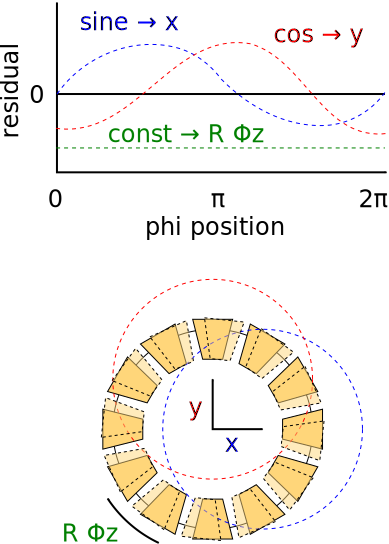
\includegraphics[width=\linewidth]{tracker_disk_interpretation.pdf}

\column{0.6\linewidth}
\includegraphics[height=\linewidth, angle=90]{ringfits_before_mem12.pdf}

\includegraphics[height=\linewidth, angle=90]{ringfits_after_mem12.pdf}
\end{columns}
\end{frame}

\begin{frame}
\frametitle{Table of ring corrections}
\begin{itemize}
\item Track-based corrections with respect to design geometry
\item Grouped items are physically connected to the same disk; \\ values are correlated but not exactly equal within fitting errors
\end{itemize}

\vspace{-0.5 cm}
\begin{center}
\scriptsize
\renewcommand{\arraystretch}{1.1}
\begin{tabular}{c | c c c}
ring & $\delta_x$ (mm) & $\delta_y$ (mm) & $\delta_{\phi_z}$ (mrad) \\\hline
ME$-$4/1 & $ 5.00$ $\pm$ $ 0.14$ & $-1.30$ $\pm$ $ 0.22$ & $ 1.57$ $\pm$ $ 0.05$ \\\hline
ME$-$3/2 & $ 2.25$ $\pm$ $ 0.04$ & $-0.62$ $\pm$ $ 0.06$ & $ 1.85$ $\pm$ $ 0.01$ \\
ME$-$3/1 & $ 4.16$ $\pm$ $ 0.12$ & $ 0.06$ $\pm$ $ 0.18$ & $ 2.12$ $\pm$ $ 0.04$ \\
ME$-$2/2 & $ 1.66$ $\pm$ $ 0.04$ & $ 1.29$ $\pm$ $ 0.05$ & $ 1.68$ $\pm$ $ 0.01$ \\
ME$-$2/1 & $ 3.77$ $\pm$ $ 0.09$ & $-1.96$ $\pm$ $ 0.13$ & $ 2.18$ $\pm$ $ 0.03$ \\\hline
ME$-$1/3 & $ 2.41$ $\pm$ $ 0.06$ & $ 1.43$ $\pm$ $ 0.09$ & $ 0.26$ $\pm$ $ 0.01$ \\
ME$-$1/2 & $ 3.52$ $\pm$ $ 0.05$ & $-1.56$ $\pm$ $ 0.07$ & $ 0.85$ $\pm$ $ 0.01$ \\
ME$-$1/1 & $ 2.93$ $\pm$ $ 0.09$ & $-2.90$ $\pm$ $ 0.13$ & $ 0.66$ $\pm$ $ 0.04$ \\\hline
ME$+$1/1 & $ 4.95$ $\pm$ $ 0.08$ & $-1.93$ $\pm$ $ 0.11$ & $ 0.17$ $\pm$ $ 0.04$ \\
ME$+$1/2 & $ 5.05$ $\pm$ $ 0.05$ & $ 0.81$ $\pm$ $ 0.07$ & $ 0.13$ $\pm$ $ 0.01$ \\
ME$+$1/3 & $ 4.36$ $\pm$ $ 0.06$ & $ 3.22$ $\pm$ $ 0.08$ & $ 0.02$ $\pm$ $ 0.01$ \\\hline
ME$+$2/1 & $ 4.56$ $\pm$ $ 0.08$ & $ 2.30$ $\pm$ $ 0.12$ & $ 0.18$ $\pm$ $ 0.03$ \\
ME$+$2/2 & $ 4.28$ $\pm$ $ 0.04$ & $ 3.86$ $\pm$ $ 0.05$ & $-0.11$ $\pm$ $ 0.01$ \\
ME$+$3/1 & $ 5.06$ $\pm$ $ 0.10$ & $ 4.42$ $\pm$ $ 0.17$ & $-0.05$ $\pm$ $ 0.03$ \\
ME$+$3/2 & $ 4.01$ $\pm$ $ 0.04$ & $ 4.88$ $\pm$ $ 0.06$ & $-0.37$ $\pm$ $ 0.01$ \\\hline
ME$+$4/1 & $ 5.58$ $\pm$ $ 0.15$ & $ 8.24$ $\pm$ $ 0.24$ & $ 0.40$ $\pm$ $ 0.05$ \\
\end{tabular}
\end{center}
\end{frame}

\begin{frame}
\frametitle{Ring fits with collisions}

\begin{itemize}
\item Collisions muons will cover the inner rings better than cosmics
\item MC resolution estimate:
\end{itemize}

\includegraphics[height=\linewidth, angle=90]{mccsc_example_5pb.pdf}

\hfill \includegraphics[height=0.45\linewidth, angle=90]{mccsc_diskstats_xy.pdf}\includegraphics[height=0.45\linewidth, angle=90]{mccsc_diskstats_phiz.pdf}
\end{frame}

\begin{frame}
\frametitle{Problem in tracker-to-CSC}

\begin{columns}
\column{0.7\linewidth}
\includegraphics[width=\linewidth]{cscringproblem_40gev.png}

\includegraphics[width=\linewidth]{cscringproblem_100gev.png}

\column{0.4\linewidth}
\begin{itemize}
\item Residuals on low-$p_T$ tracks alternate unphysically between chambers; not so for high-$p_T$ tracks

\item Dashed lines are chamber boundaries \\ (4 bins per chamber)

\item Corresponding effect {\it not} seen in overlaps

\item This is a very weird effect: defies most explanations (full detective story not shown here)

\item \mbox{Continued next page\ldots\hspace{-1 cm}}
\end{itemize}
\end{columns}
\end{frame}

\begin{frame}
\frametitle{New alignment expert}
\framesubtitle{(in training)}

\begin{itemize}
\item \textcolor{darkblue}{Aysen Tatarinov}, new grad student at Texas A\&M, will be taking on alignment responsibilities

\item Current status: I've documented all of the tools on twiki pages

{\tiny https://twiki.cern.ch/twiki/bin/view/CMS/SWGuideMuonAlignment

\textcolor{white}{https://twiki.cern.ch/twiki/bin/view/CMS/}SWGuideMuonAlignReferenceTarget

\textcolor{white}{https://twiki.cern.ch/twiki/bin/view/CMS/}SWGuideMuonAlignFrameworkDetails

\textcolor{white}{https://twiki.cern.ch/twiki/bin/view/CMS/}SWGuideMuonGeometryConversion

\textcolor{white}{https://twiki.cern.ch/twiki/bin/view/CMS/}SWGuideMuonGeometryDBComparison

\textcolor{white}{https://twiki.cern.ch/twiki/bin/view/CMS/}SWGuideMuonAlignValidationPlots

\textcolor{white}{https://twiki.cern.ch/twiki/bin/view/CMS/}FindQualityFilesPy

\textcolor{white}{https://twiki.cern.ch/twiki/bin/view/CMS/}SWGuideMuonAlignStandAloneTest

\textcolor{white}{https://twiki.cern.ch/twiki/bin/view/CMS/}SWGuideMuonAlignCustomGeometry

\mbox{ }}

\vspace{-0.5 cm}
and he is successfully using them to produce MC alignment results

\item First major project will be to solve the CSC residuals problem shown on the previous page (with help from me)

\item \textcolor{darkblue}{Vadim Khotilovich} is also still developing infrastructure \\ Completed: FindQualityFiles, next project: \mbox{unified monitoring system\hspace{-1 cm}}
\end{itemize}
\end{frame}

\begin{frame}
\frametitle{Step 3: Reference-Target}

\begin{itemize}
\item High-luminosity: align each chamber individually using tracks from the tracker

\item Any discrepancies between this and overlaps alignment will tell us a lot about tracker or track-propagation errors

\item Simulation produced by Aysen: 50~pb$^{-1}$ yields 320~$\mu$m in $r\phi$, comparable to beam-halo resolution, enough to make a good test
\begin{itemize}
\item now trying 5, 10, and 20~pb$^{-1}$
\end{itemize}
\end{itemize}

\begin{center}
\includegraphics[width=0.8\linewidth]{only3_CSC.png}
\end{center}
\end{frame}


%% \section*{First section}
%% \begin{frame}
%% \begin{center}
%% \Huge \textcolor{blue}{First section}
%% \end{center}
%% \end{frame}

\begin{frame}
\frametitle{Conclusions}
\begin{itemize}\setlength{\itemsep}{0.5 cm}
\item Beam-induced muons have arrived, but not yet in great numbers like last year (clean beams, cautious with inner-ring CSC voltage)

\item The events that we do have look very promising

\item We have aligned rings relative to the tracker using CRAFT-09 cosmic rays; extends naturally to early collisions

\item Ring alignment revealed a very strange feature

\item Aysen is joining us in the alignment effort: his first major task will be understanding the very strange feature

\end{itemize}
\label{numpages}
\end{frame}

\end{document}
